\documentclass[12pt,a4paper,oneside]{report}

% ==============================================================================
% PACKAGES & CONFIGURATION
% ==============================================================================
\usepackage[utf8]{inputenc}
\usepackage[T1]{fontenc}
\usepackage{lmodern}
\usepackage[english]{babel}
\usepackage[margin=2.5cm,top=2.5cm,bottom=2.5cm,headheight=15pt]{geometry}
\usepackage{graphicx}
\usepackage{xcolor}
\usepackage{amsmath,amssymb}
\usepackage{booktabs}
\usepackage{tabularx}
\usepackage{multirow}
\usepackage{listings}
\usepackage{fancyhdr}
\usepackage{titlesec}
\usepackage{tikz}
\usetikzlibrary{shapes.geometric, arrows.meta, positioning, calc, fit, backgrounds, shadows}
\usepackage[hidelinks,pdfusetitle]{hyperref}
\usepackage{microtype}
\usepackage{setspace}
\usepackage{caption}
\usepackage{subcaption}
\usepackage{csquotes}

% Colors definition
\definecolor{primaryblue}{RGB}{18, 52, 102}      % EHTP / 2M Navy Blue
\definecolor{secondaryblue}{RGB}{30, 100, 180}   % Royal Blue
\definecolor{accentorange}{RGB}{235, 110, 30}    % LionGeek Accent Orange
\definecolor{darkgray}{RGB}{50, 50, 50}
\definecolor{lightgray}{RGB}{245, 247, 250}
\definecolor{codebg}{RGB}{248, 249, 250}
\definecolor{codeframe}{RGB}{220, 224, 230}

% Code Listings Configuration
\lstset{
    backgroundcolor=\color{codebg},
    basicstyle=\ttfamily\footnotesize\color{darkgray},
    keywordstyle=\bfseries\color{primaryblue},
    stringstyle=\color{accentorange},
    commentstyle=\itshape\color{gray},
    numbers=left,
    numberstyle=\tiny\color{gray},
    stepnumber=1,
    numbersep=8pt,
    frame=single,
    rulecolor=\color{codeframe},
    breaklines=true,
    breakatwhitespace=true,
    tabsize=2,
    showstringspaces=false,
    captionpos=b
}

% Typography & Spacing
\onehalfspacing
\setlength{\parskip}{6pt}
\setlength{\parindent}{0pt}

% Header & Footer Styling
\pagestyle{fancy}
\fancyhf{}
\fancyhead[L]{\small\scshape\color{darkgray} GridCast --- LionGeek / 2M Internship Report}
\fancyhead[R]{\small\color{darkgray}\thepage}
\fancyfoot[C]{\footnotesize\color{gray} Hassania School of Public Works (EHTP) --- Academic Year 2025/2026}
\renewcommand{\headrulewidth}{0.4pt}
\renewcommand{\footrulewidth}{0.4pt}

% Chapter & Section title formatting
\titleformat{\chapter}[display]
{\normalfont\huge\bfseries\color{primaryblue}}{\filleft\Huge\color{accentorange}\chaptertitlename\ \thechapter}{10pt}
{\titlerule[1.5pt]\vspace{6pt}\filright}[\vspace{6pt}\titlerule]

\titleformat{\section}
{\normalfont\Large\bfseries\color{secondaryblue}}{\thesection}{1em}{}

\titleformat{\subsection}
{\normalfont\large\bfseries\color{primaryblue}}{\thesubsection}{1em}{}

\begin{document}

% ==============================================================================
% COVER PAGE (INSPIRED BY EHTP & 2M TRADITIONAL LAYOUT)
% ==============================================================================
\begin{titlepage}
\begin{tikzpicture}[remember picture,overlay]
    \draw[line width=1.5pt, color=primaryblue] 
        ($(current page.north west) + (1.5cm,-1.5cm)$) 
        rectangle 
        ($(current page.south east) + (-1.5cm,1.5cm)$);
    \draw[line width=0.5pt, color=accentorange] 
        ($(current page.north west) + (1.65cm,-1.65cm)$) 
        rectangle 
        ($(current page.south east) + (-1.65cm,1.65cm)$);
\end{tikzpicture}

\centering
\vspace*{-0.5cm}

{\scshape\bfseries\large KINGDOM OF MOROCCO}\\[0.2cm]
{\scshape\bfseries\normalsize Ministry of Equipment, Transport, Logistics and Water}\\[0.2cm]
{\scshape\bfseries\large HASSANIA SCHOOL OF PUBLIC WORKS (EHTP)}\\[0.2cm]
{\scshape\normalsize Department of Computer Science \& Telecommunications}\\[0.6cm]

\begin{center}
    \begin{tabular}{cc}
        \textbf{\large LIONGEEK} & \textbf{\large SOREAD 2M} \\
        \textit{\small Digital Innovation Hub \& Tech Incubator} & \textit{\small National Television Broadcaster}
    \end{tabular}
\end{center}

\vspace{0.8cm}
{\color{accentorange}\rule{0.85\textwidth}{2pt}}\\[0.4cm]
{\LARGE\bfseries\color{primaryblue} INTERNSHIP REPORT}\\[0.3cm]
{\large\bfseries Degree of State Engineer in Computer Science}\\[0.4cm]
{\color{accentorange}\rule{0.85\textwidth}{2pt}}\\[0.8cm]

{\LARGE\bfseries\color{primaryblue} DESIGN AND IMPLEMENTATION OF GRIDCAST:}\\[0.3cm]
{\Large\bfseries An Audiovisual TV Broadcast Grid Management Platform with an Intelligent AI Assistant and a DevOps Deployment Architecture}\\[1.0cm]

\begin{minipage}{0.48\textwidth}
    \textbf{Prepared by:}\\[0.2cm]
    \textbf{Student Engineer}\\[0.1cm]
    \textit{EHTP Casablanca}
\end{minipage}
\hfill
\begin{minipage}{0.48\textwidth}
    \begin{flushright}
    \textbf{Supervised by:}\\[0.2cm]
    \textbf{Prof. Academic Supervisor} (EHTP)\\[0.1cm]
    \textbf{Eng. Professional Mentor} (LionGeek / 2M)
    \end{flushright}
\end{minipage}

\vfill
\textbf{Host Institution:} LionGeek (Innovation Hub \& Subsidiary of SOREAD 2M, Casablanca)\\[0.2cm]
\textbf{Internship Period:} 2 Months (July -- August 2025)\\[0.2cm]
\textbf{Academic Year:} 2025 -- 2026

\end{titlepage}

% ==============================================================================
% DEDICATION & ACKNOWLEDGMENTS
% ==============================================================================
\pagenumbering{roman}
\setcounter{page}{1}

\chapter*{Acknowledgments}
\addcontentsline{toc}{chapter}{Acknowledgments}

First and foremost, I express my sincere gratitude and deep appreciation to the entire technical and managerial leadership of \textbf{LionGeek}, the digital innovation hub and incubator of \textbf{SOREAD 2M}. Hosting me within this vibrant and forward-thinking environment provided an exceptional setting for professional and technical maturation.

I would like to address my profound thankfulness to my company supervisor and mentor at LionGeek, whose high standards, guidance, and continuous trust enabled me to take ownership of complex technical challenges, from modern full-stack engineering to cloud deployment strategies. I am equally thankful to the software engineering team at LionGeek and 2M for their warm integration, constructive technical feedback, and stimulating architectural discussions throughout these two intense months.

I am deeply grateful to my academic supervisor, whose pedagogy, rigor, and technical advice guided my approach to modeling, software engineering discipline, and formal reporting. 

My heartfelt appreciation extends to the administrative and teaching staff of the \textbf{Department of Computer Science and Telecommunications} at the \textbf{Hassania School of Public Works (EHTP)}. The solid engineering curriculum and academic grounding instilled during our education formed the indispensable foundation upon which this internship was executed.

Lastly, I express my deepest love and gratitude to my family and colleagues for their unwavering support, patience, and encouragement throughout my academic journey.

\vspace{1.5cm}
\begin{flushright}
    \textit{The Student Engineer}\\
    \textit{Casablanca, Morocco}
\end{flushright}

\newpage

% ==============================================================================
% EXECUTIVE SUMMARY & RESUME
% ==============================================================================
\chapter*{Abstract \& Résumé}
\addcontentsline{toc}{chapter}{Abstract \& Résumé}

\section*{Abstract}
This report documents a two-month engineering internship carried out at \textbf{LionGeek}, the technological subsidiary and digital innovation incubator of the national broadcaster \textbf{SOREAD 2M} in Casablanca, Morocco. The core assignment revolved around the design, full-stack development, and deployment of \textbf{GridCast}, a mission-critical web platform engineered to modernize television programming grid management, audiovisual content cataloging, advertising slot pricing, and audience analytics. 

During the internship, the first two weeks were structured as an intensive on-site technical deep dive, where the official documentation and state-of-the-art standards of \textbf{Laravel 12}, \textbf{Inertia.js v2}, \textbf{React 19}, \textbf{TypeScript}, and \textbf{Tailwind CSS v4} were mastered in depth, complementing the foundational Artificial Intelligence competencies acquired academically at EHTP. Furthermore, the intern contributed to a secondary high-priority enterprise project that remains confidential due to non-disclosure obligations.

To address the broadcast scheduling requirements, a comprehensive UML conception was established, incorporating strict temporal interval non-overlap validation algorithms, role-based workflows for producers and programming executives, and financial yield calculations for advertising. Additionally, an intelligent \textbf{AI Chatbot Assistant (GridCast AI)} powered by Google Gemini 2.5 Flash was embedded with dynamic live-database context injection (Retrieval-Augmented Generation), enabling real-time conversational inquiries in Arabic, Darija, and French. Finally, a production-grade \textbf{DevOps pipeline} was designed, including multi-stage Docker containerization, automated CI/CD testing with Pest PHP and Laravel Pint, and Nginx reverse proxy hardening.

\textbf{Keywords:} Broadcast Scheduling, SOREAD 2M, LionGeek, Laravel 12, Inertia.js v2, React 19, TypeScript, Generative AI Chatbot, RAG, UML Modeling, Docker, CI/CD, DevOps.

\vspace{0.8cm}
\hrule
\vspace{0.8cm}

\section*{Résumé (Français)}
Ce rapport présente le travail accompli durant un stage d'ingénieur de deux mois au sein de \textbf{LionGeek}, incubateur et filiale technologique de la chaîne nationale \textbf{SOREAD 2M}. Le projet majeur porte sur la conception, la réalisation et le déploiement de \textbf{GridCast}, une plateforme web de gestion de grille de programmes télévisuels, de gestion de catalogue multi-langues (Arabe, Darija, Français), de régie publicitaire et de suivi d'audience.

Les deux premières semaines ont été consacrées à une étude en présentiel approfondie de la documentation de Laravel 12, Inertia.js v2, React 19, TypeScript et Tailwind CSS v4. Le stagiaire a également collaboré sur un projet stratégique interne couvert par le secret professionnel. Le système intègre un assistant conversationnel intelligent fondé sur l'IA générative (Gemini 2.5 Flash) exploitant les données de diffusion en temps réel, une modélisation UML rigoureuse (anti-chevauchement des créneaux) ainsi qu'un pipeline complet DevOps (Docker, CI/CD GitHub Actions, Nginx).

\textbf{Mots-clés :} Grille TV, SOREAD 2M, LionGeek, Laravel, Inertia, React, Chatbot IA, RAG, UML, DevOps.

\newpage

% ==============================================================================
% LIST OF ABBREVIATIONS
% ==============================================================================
\chapter*{List of Abbreviations}
\addcontentsline{toc}{chapter}{List of Abbreviations}

\begin{table}[h!]
\centering
\begin{tabularx}{\textwidth}{llX}
\toprule
\textbf{Abbreviation} & \textbf{Term} & \textbf{Meaning / Definition} \\
\midrule
\textbf{EHTP} & École Hassania des Travaux Publics & Moroccan National Engineering Grande École \\
\textbf{2M / SOREAD} & Société d'Études et de Réalisations Audiovisuelles & National Public Television Broadcaster of Morocco \\
\textbf{SPA} & Single-Page Application & Client-side web application dynamic rendering \\
\textbf{SSR} & Server-Side Rendering & Pre-rendering web markup on the server \\
\textbf{MVC} & Model-View-Controller & Architectural design pattern \\
\textbf{ORM} & Object-Relational Mapping & Eloquent database abstraction layer in Laravel \\
\textbf{API} & Application Programming Interface & Interface for inter-system communication \\
\textbf{REST} & Representational State Transfer & Stateless architectural style for APIs \\
\textbf{RAG} & Retrieval-Augmented Generation & Supplementing LLMs with live database context \\
\textbf{LLM} & Large Language Model & Foundation artificial intelligence model \\
\textbf{UML} & Unified Modeling Language & Standard visual modeling language for software \\
\textbf{ERD} & Entity-Relationship Diagram & Database conceptual data model \\
\textbf{CI/CD} & Continuous Integration / Continuous Deployment & Automated software build, test, and release cycle \\
\textbf{PST} & Prime-Time Slot & Peak television broadcast viewing hours \\
\textbf{JT} & Journal Télévisé & Television News Broadcast \\
\textbf{CSRF} & Cross-Site Request Forgery & Web security protection mechanism \\
\bottomrule
\end{tabularx}
\end{table}

\newpage

% ==============================================================================
% TABLE OF CONTENTS & LISTS
% ==============================================================================
\tableofcontents
\newpage
\listoffigures
\newpage
\listoftables
\newpage

\pagenumbering{arabic}
\setcounter{page}{1}


% ==============================================================================
% CHAPTER 1: GENERAL CONTEXT AND HOST ORGANIZATION
% ==============================================================================
\chapter{General Context and Host Organization}
\label{chap:context}

\section{Introduction}
Television broadcasting operates within a rigorous, real-time environment where milliseconds govern transmission schedules, programming conflicts cause catastrophic on-air downtime, and advertising revenue hinges upon audience precision. In modern television stations, transitioning from archaic, paper-based or decoupled spreadsheet planning to a unified, distributed, and automated broadcast management platform represents a strategic imperative. This report chronicles an engineering endeavor conducted at \textbf{LionGeek}, the technological arm of \textbf{SOREAD 2M}, aiming to conceptualize, engineer, and deploy \textbf{GridCast}---an enterprise television grid and audiovisual scheduling system augmented by Artificial Intelligence.

\section{Host Organization: SOREAD 2M and LionGeek}

\subsection{SOREAD 2M: The National Broadcasting Pillar}
Established in 1989 as the first private pay-TV channel in the Arab-African region before transitioning into a public-service television broadcaster in 1996, \textbf{SOREAD 2M} (Société d'Études et de Réalisations Audiovisuelles) stands as Morocco's leading generalist television station. Broadcasting across terrestrial and satellite channels in high definition (HD), 2M serves over 30 million domestic viewers alongside a vast diaspora across Europe, North America, and the Middle East.

A defining characteristic of 2M is its trilingual broadcast identity. Its broadcast schedules interweave three distinct linguistic vehicles:
\begin{itemize}
    \item \textbf{Standard Arabic (ar):} Utilized for formal news bulletins (\textit{Al Massaiya}), national debates, and religious broadcasts.
    \item \textbf{Moroccan Darija (darija):} The primary cultural medium for prime-time soap operas (\textit{Dar Lghizlane}), sitcoms, comedy sketches, and Botola Pro football league commentary.
    \item \textbf{French (fr):} Employed for analytical documentary series (\textit{Grand Angle Maroc}), investigative reporting, and economic forums.
\end{itemize}

Managing this multidimensional ecosystem requires synchronized alignment between content creators, commissioning editors, advertising agencies, and transmission engineers.

\subsection{LionGeek: The Digital Hub \& Innovation Incubator}
\textbf{LionGeek} is the technological subsidiary and innovation factory launched by SOREAD 2M in Casablanca. Situated at the nexus of media and software engineering, LionGeek operates as an incubation campus, technological incubator, and internal digital production agency. Its mission is to drive digital transformation across Moroccan broadcasting, accelerate emerging engineering talent, and incubate next-generation media technologies such as streaming platforms, telemetry engines, and workflow automation.

\begin{figure}[h!]
\centering
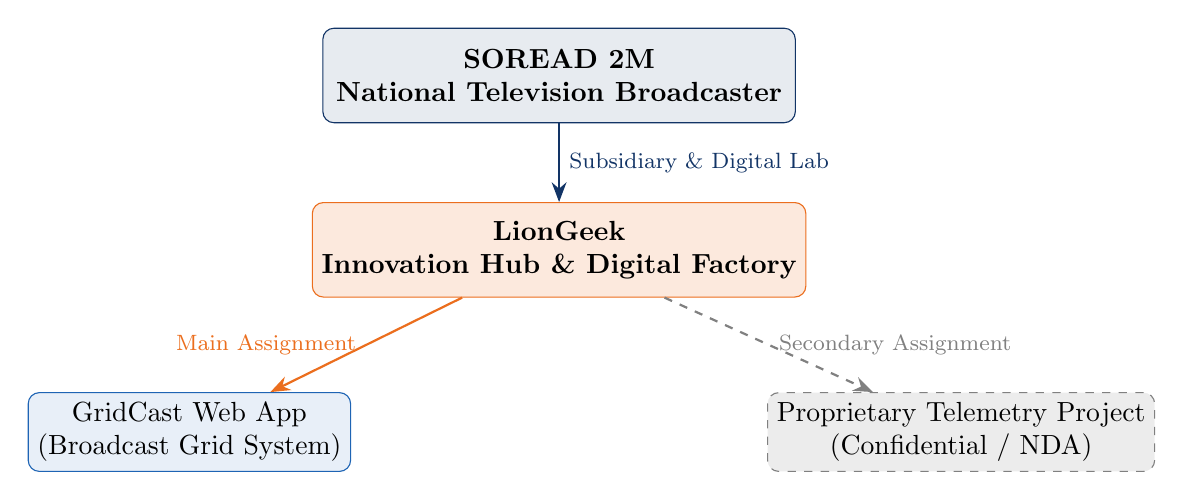
\begin{tikzpicture}[node distance=1.5cm, auto]
    \node (soread) [draw=primaryblue, fill=primaryblue!10, rounded corners, minimum width=6cm, minimum height=1.2cm, align=center, font=\bfseries] {SOREAD 2M\\National Television Broadcaster};
    \node (liongeek) [draw=accentorange, fill=accentorange!15, rounded corners, minimum width=5cm, minimum height=1.2cm, below=1cm of soread, align=center, font=\bfseries] {LionGeek\\Innovation Hub \& Digital Factory};
    \node (gridcast) [draw=secondaryblue, fill=secondaryblue!10, rounded corners, minimum width=4cm, minimum height=1cm, below left=1.2cm and -0.5cm of liongeek, align=center] {GridCast Web App\\(Broadcast Grid System)};
    \node (confidential) [draw=gray, fill=gray!15, rounded corners, minimum width=4cm, minimum height=1cm, below right=1.2cm and -0.5cm of liongeek, align=center, dashed] {Proprietary Telemetry Project\\(Confidential / NDA)};

    \draw[-{Stealth[length=2.5mm]}, thick, color=primaryblue] (soread) -- (liongeek) node[midway, right, font=\footnotesize] {Subsidiary \& Digital Lab};
    \draw[-{Stealth[length=2.5mm]}, thick, color=accentorange] (liongeek) -- (gridcast) node[midway, left, font=\footnotesize] {Main Assignment};
    \draw[-{Stealth[length=2.5mm]}, thick, color=gray, dashed] (liongeek) -- (confidential) node[midway, right, font=\footnotesize] {Secondary Assignment};
\end{tikzpicture}
\caption{Organizational Hierarchy and Project Distribution at LionGeek / 2M}
\label{fig:org_chart}
\end{figure}

\section{Internship Framework and Timeline}
The internship spanned an intensive two-month period during the summer term. The schedule was structured into well-defined phases designed to maximize technical mastery and operational impact.

\subsection{Phase 1: Weeks 1--2 --- Intensive Technical Onboarding}
The first two weeks were conducted on-site at LionGeek's Casablanca headquarters as a dedicated technical immersion. Recognizing that television grid operations require resilient and modern web architectures, LionGeek mentors mandated a thorough review and deep dive into the official technical documentation of the target stack:
\begin{enumerate}
    \item \textbf{Laravel 12 (Backend Architecture):} Thorough study of Eloquent ORM relations, Form Request lifecycle, Policy-driven authorization gates, database transactions, and custom validation rules.
    \item \textbf{Inertia.js v2 (Monolithic SPA Bridge):} Deep dive into the server-driven Single-Page Application paradigm, examining how Inertia eliminates the boilerplate of REST APIs by passing server-side Eloquent data directly into React page components via shared props.
    \item \textbf{React 19 \& TypeScript:} Rigorous exploration of strict TypeScript typing interfaces, functional components, hooks (\texttt{useForm}, \texttt{usePage}), and state reconciliation.
    \item \textbf{Tailwind CSS v4:} Mastery of the updated PostCSS engine, custom CSS variables, and clean enterprise user interface patterns.
    \item \textbf{Quality Tooling:} Configuration and enforcement of PSR-12 code standards through Laravel Pint, as well as ESLint and Prettier for the frontend.
\end{enumerate}

\begin{quote}
\textit{Academic Foundation Clarification:} It is important to emphasize that while modern full-stack web engineering frameworks were internalized during this initial on-site immersion at LionGeek, the foundational principles of Artificial Intelligence, Natural Language Processing, and LLM integrations leveraged in this project were acquired through previous coursework at the Hassania School of Public Works (EHTP).
\end{quote}

\subsection{Dual Project Context and Confidentiality Clause}
During the two-month tenure, the intern was assigned to contribute across two enterprise initiatives:
\begin{itemize}
    \item \textbf{Confidential Digital Telemetry Project:} A proprietary backend infrastructure initiative handling internal streaming traffic analytics and audience telemetry. Due to strict non-disclosure agreements (NDA) protecting SOREAD 2M internal intellectual property, the technical artifacts of this secondary project cannot be detailed within this public document.
    \item \textbf{GridCast (Primary Project):} The complete design, implementation, and deployment of the next-generation TV broadcast planning, advertising monetization, and AI-assisted scheduling system. This open project forms the comprehensive subject of this report.
\end{itemize}

\subsection{Problem Statement and Motivation}
Historically, television scheduling at large broadcast stations suffered from operational bottlenecks:
\begin{itemize}
    \item \textbf{Schedule Overlap Catastrophes:} Planning slots manually across different transmission zones risked double-booking time intervals. An overlap directly causes on-air transmission failure.
    \item \textbf{Fragmented Producer Workflow:} External audiovisual producers submitted tape reels and metadata through disconnected channels (emails, physical drives), with no centralized status tracking (Draft $\rightarrow$ Submitted $\rightarrow$ Validated/Rejected).
    \item \textbf{Decoupled Advertising Reconciliation:} The commercial advertising department lacked live synchronization with planned program lengths, leading to unsold commercial breaks or delayed spot broadcast certifications.
    \item \textbf{Information Asymmetry:} Station executives lacked rapid, conversational access to real-time grid metrics, remaining dependent on static end-of-week PDF reports.
\end{itemize}
These limitations motivated the development of \textbf{GridCast}.


% ==============================================================================
% CHAPTER 2: PROJECT SPECIFICATIONS AND REQUIREMENTS ANALYSIS
% ==============================================================================
\chapter{Project Specifications and Requirements Analysis}
\label{chap:specs}

\section{Introduction}
Developing an enterprise broadcast platform necessitates mapping business operations into unambiguous technical requirements. This chapter formalizes the functional and non-functional requirements governing GridCast.

\section{Actors and Stakeholder Profiles}
The system models four primary operational actors, enforced through server-side role-based access control (RBAC):
\begin{enumerate}
    \item \textbf{Programming Manager (Responsable Programmation):} Responsible for scheduling weekly broadcast grids, defining transmission zones, and reviewing producer submissions.
    \item \textbf{Audiovisual Producer (Producteur / Réalisateur):} Submits new television shows, series, and episode metadata, tracks validation statuses, and revises rejected submissions.
    \item \textbf{Advertising Department (Régie Publicitaire):} Manages corporate commercial clients (e.g., Maroc Telecom, inwi, Orange), books advertising spots onto planned tunnels, and tracks financial yield.
    \item \textbf{Station Administrator (Administrateur):} Holds overarching governance over users, global system categories, and executive analytics dashboards.
\end{enumerate}

\begin{table}[h!]
\centering
\caption{Actor Matrix and Operational Permissions}
\label{tab:actors_matrix}
\begin{tabularx}{\textwidth}{lXX}
\toprule
\textbf{Role} & \textbf{Core Permissions} & \textbf{Business Objective} \\
\midrule
\texttt{admin} & Full system CRUD, user management, global analytics & Platform governance \& executive monitoring \\
\texttt{programmation} & Validation queue, weekly calendar drag-and-drop & Grid optimization \& schedule conflict prevention \\
\texttt{producteur} & Draft programs, submit episodes, view feedback & Content onboarding \& production lifecycle \\
\texttt{regie} & Manage advertisers, book ad slots, monitor billing & Commercial revenue maximization \\
\bottomrule
\end{tabularx}
\end{table}

\section{Functional Requirements (FR)}
The functional landscape is categorized into six fundamental modules:

\begin{itemize}
    \item \textbf{FR1: Broadcast Grid Management \& Non-Overlap Engine}
    \begin{itemize}
        \item The system shall present an interactive weekly grid calendar (Monday to Sunday) segmented into 24-hour time slots and channel zones (Prime Time, Access, Matinée, Nuit).
        \item The system shall provide an intuitive drag-and-drop interface allowing real-time slot rescheduling.
        \item \textbf{Core Business Rule:} The backend must strictly reject any broadcast slot that temporally overlaps with an existing slot within the same channel zone.
    \end{itemize}

    \item \textbf{FR2: Audiovisual Program Catalog}
    \begin{itemize}
        \item The catalog shall index programs with titles, synopsis, duration in minutes, categories, and production credits.
        \item Support multi-language broadcasting metadata: Arabic (\texttt{ar}), Moroccan Darija (\texttt{darija}), and French (\texttt{fr}).
        \item Provide instant search, category filtering, and pagination without full page reloads.
    \end{itemize}

    \item \textbf{FR3: Producer Submission Lifecycle (State Machine)}
    \begin{itemize}
        \item Programs follow a deterministic lifecycle: \texttt{brouillon} (Draft) $\rightarrow$ \texttt{soumis} (Submitted) $\rightarrow$ \texttt{valide} (Approved) or \texttt{rejete} (Rejected).
        \item Only valid state transitions shall be permitted; producers can edit only draft or rejected programs.
        \item Automated database notifications alert producers upon review decisions.
    \end{itemize}

    \item \textbf{FR4: Advertising Monetization and Commercial Slots}
    \begin{itemize}
        \item Register corporate advertisers with contact information and contractual notes.
        \item Reserve advertising slots tied to scheduled broadcast windows or autonomous tunnels.
        \item Calculate aggregate revenue (e.g., in Moroccan Dirhams --- MAD) per broadcast cycle.
    \end{itemize}

    \item \textbf{FR5: Executive Audience Analytics Dashboard}
    \begin{itemize}
        \item Aggregate audience ratings (viewers, market share percentage) across broadcast zones.
        \item Render real-time charts (category distribution, approval ratios, revenue breakdown).
    \end{itemize}

    \item \textbf{FR6: Embedded Real-Time AI Chatbot Assistant}
    \begin{itemize}
        \item Provide an always-available floating assistant (\textbf{GridCast AI}) powered by Gemini 2.5 Flash.
        \item The chatbot must dynamically query the live database state (RAG context injection) to answer specific questions regarding scheduled shows, ad revenue, and pending submissions.
        \item Deliver fluent responses in French, Darija, and Arabic.
    \end{itemize}
\end{itemize}

\section{Non-Functional Requirements (NFR)}
\begin{itemize}
    \item \textbf{Security:} Enforce Cross-Site Request Forgery (CSRF) protection on all state mutations, password hashing via Bcrypt (rounds = 12), and role validation middleware at the kernel level.
    \item \textbf{Performance:} Page transitions within Inertia.js must execute in under 300ms by exchanging JSON payloads rather than re-rendering complete HTML DOM trees.
    \item \textbf{Code Quality:} Backend code must strictly comply with the PSR-12 standard verified via Laravel Pint. Frontend code must compile cleanly through ESLint with zero TypeScript errors.
\end{itemize}


% ==============================================================================
% CHAPTER 3: SYSTEM CONCEPTION AND UML MODELING
% ==============================================================================
\chapter{System Conception and UML Modeling}
\label{chap:conception}

\section{Introduction}
Software modeling provides the blueprint connecting real-world broadcast operations with object-oriented software architectures. This chapter develops the complete conceptual design of GridCast using the Unified Modeling Language (UML).

\section{Methodological Approach: Agile-Scrum \& UML}
The project adopted an Agile-Scrum methodology structured in two-week sprints. Requirements were modeled using UML to provide visual verification of functional dependencies and database normalization prior to coding.

\section{Global Context Diagram}
The global context diagram depicts how external human actors and external cloud services interact with the boundary of GridCast.

\begin{figure}[h!]
\centering
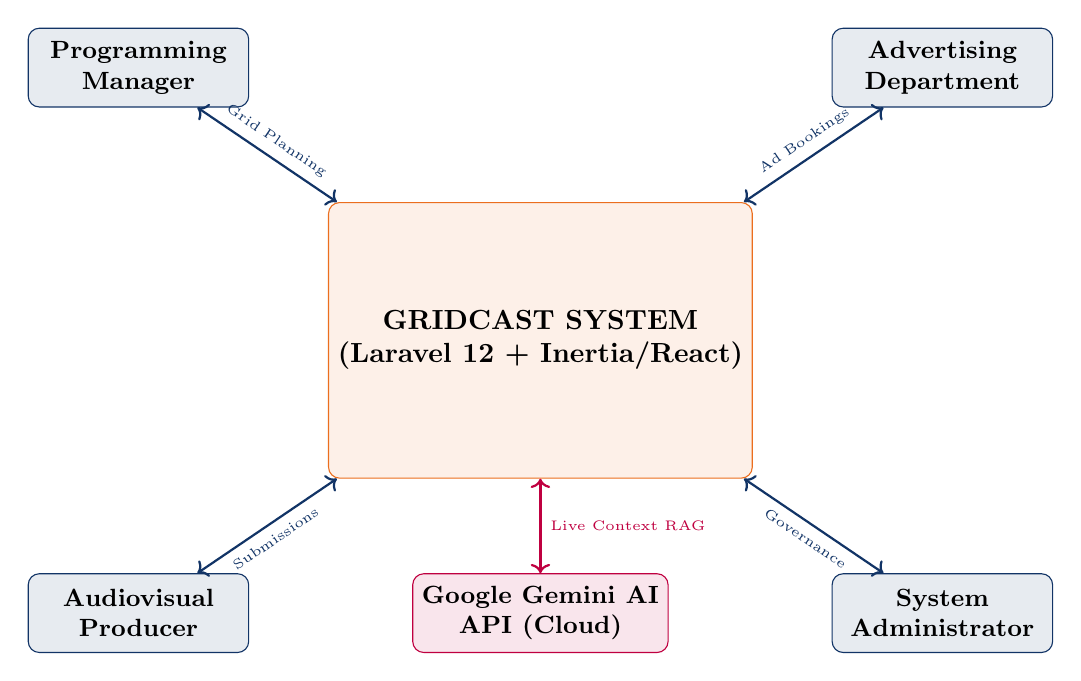
\begin{tikzpicture}[
    actor/.style={draw=primaryblue, fill=primaryblue!10, rounded corners, minimum width=2.8cm, minimum height=1cm, align=center, font=\small\bfseries},
    system/.style={draw=accentorange, fill=accentorange!10, rounded corners, minimum width=4.5cm, minimum height=3.5cm, align=center, font=\bfseries},
    external/.style={draw=purple, fill=purple!10, rounded corners, minimum width=2.8cm, minimum height=1cm, align=center, font=\small\bfseries}
]
    \node (gridcast) [system] {GRIDCAST SYSTEM\\(Laravel 12 + Inertia/React)};
    
    \node (prog) [actor, above left=1.2cm and 1cm of gridcast] {Programming\\Manager};
    \node (prod) [actor, below left=1.2cm and 1cm of gridcast] {Audiovisual\\Producer};
    \node (regie) [actor, above right=1.2cm and 1cm of gridcast] {Advertising\\Department};
    \node (admin) [actor, below right=1.2cm and 1cm of gridcast] {System\\Administrator};
    
    \node (gemini) [external, below=1.2cm of gridcast] {Google Gemini AI\\API (Cloud)};

    \draw[<->, thick, color=primaryblue] (prog) -- node[above, sloped, font=\tiny] {Grid Planning} (gridcast);
    \draw[<->, thick, color=primaryblue] (prod) -- node[below, sloped, font=\tiny] {Submissions} (gridcast);
    \draw[<->, thick, color=primaryblue] (regie) -- node[above, sloped, font=\tiny] {Ad Bookings} (gridcast);
    \draw[<->, thick, color=primaryblue] (admin) -- node[below, sloped, font=\tiny] {Governance} (gridcast);
    \draw[<->, thick, color=purple] (gridcast) -- node[right, font=\tiny] {Live Context RAG} (gemini);
\end{tikzpicture}
\caption{System Global Context Diagram}
\label{fig:context_diagram}
\end{figure}

\section{Use Case Modeling}

\subsection{Global Use Case Diagram}
Figure~\ref{fig:use_case} illustrates the principal use cases partitioned across the four system roles.

\begin{figure}[h!]
\centering
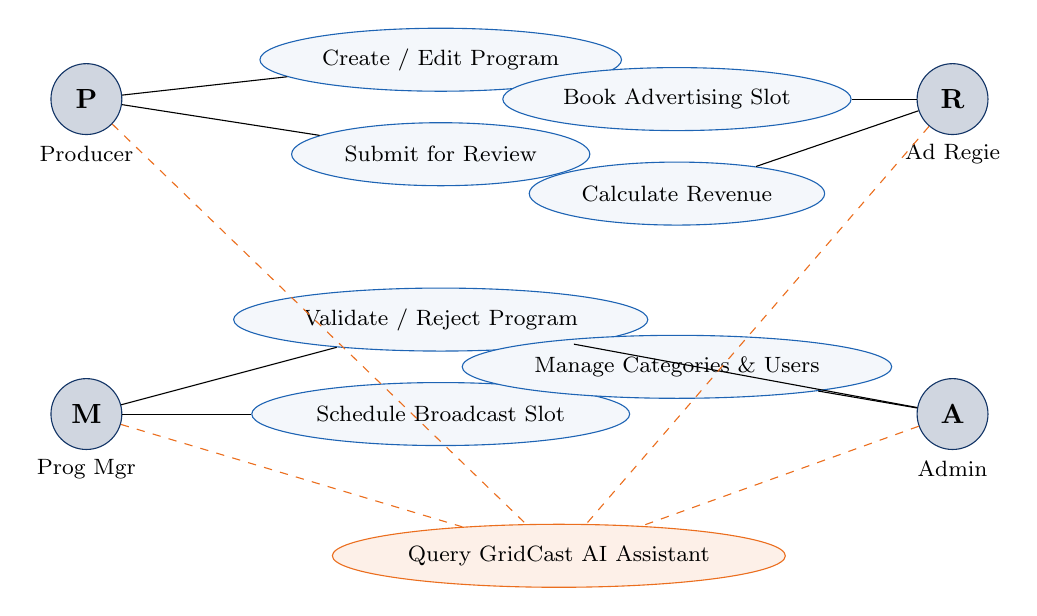
\begin{tikzpicture}[
    actor/.style={draw=primaryblue, fill=primaryblue!20, circle, minimum size=0.9cm, font=\bfseries},
    usecase/.style={draw=secondaryblue, fill=secondaryblue!5, ellipse, minimum width=3.2cm, minimum height=0.8cm, align=center, font=\footnotesize}
]
    % Actors
    \node (p_actor) [actor] at (0, 4) {P};
    \node at (0, 3.3) {\footnotesize Producer};

    \node (m_actor) [actor] at (0, 0) {M};
    \node at (0, -0.7) {\footnotesize Prog Mgr};

    \node (r_actor) [actor] at (11, 4) {R};
    \node at (11, 3.3) {\footnotesize Ad Regie};

    \node (a_actor) [actor] at (11, 0) {A};
    \node at (11, -0.7) {\footnotesize Admin};

    % Use cases
    \node (uc1) [usecase] at (4.5, 4.5) {Create / Edit Program};
    \node (uc2) [usecase] at (4.5, 3.3) {Submit for Review};
    \node (uc3) [usecase] at (4.5, 1.2) {Validate / Reject Program};
    \node (uc4) [usecase] at (4.5, 0.0) {Schedule Broadcast Slot};
    \node (uc5) [usecase] at (7.5, 4.0) {Book Advertising Slot};
    \node (uc6) [usecase] at (7.5, 2.8) {Calculate Revenue};
    \node (uc7) [usecase] at (7.5, 0.6) {Manage Categories \& Users};
    \node (uc8) [usecase, draw=accentorange, fill=accentorange!10] at (6.0, -1.8) {Query GridCast AI Assistant};

    % Associations
    \draw (p_actor) -- (uc1);
    \draw (p_actor) -- (uc2);
    \draw (m_actor) -- (uc3);
    \draw (m_actor) -- (uc4);
    \draw (r_actor) -- (uc5);
    \draw (r_actor) -- (uc6);
    \draw (a_actor) -- (uc7);
    \draw (a_actor) -- (uc3);

    % Common AI connection
    \draw[dashed, color=accentorange] (p_actor) -- (uc8);
    \draw[dashed, color=accentorange] (m_actor) -- (uc8);
    \draw[dashed, color=accentorange] (r_actor) -- (uc8);
    \draw[dashed, color=accentorange] (a_actor) -- (uc8);
\end{tikzpicture}
\caption{Global Use Case Diagram}
\label{fig:use_case}
\end{figure}

\section{Dynamic Behavioral Modeling: Sequence Diagrams}

\subsection{Sequence Diagram 1: Broadcast Slot Scheduling with Overlap Prevention}
The broadcast slot scheduling sequence ensures mathematical verification of non-overlapping intervals prior to persisting a time slot.

\begin{figure}[h!]
\centering
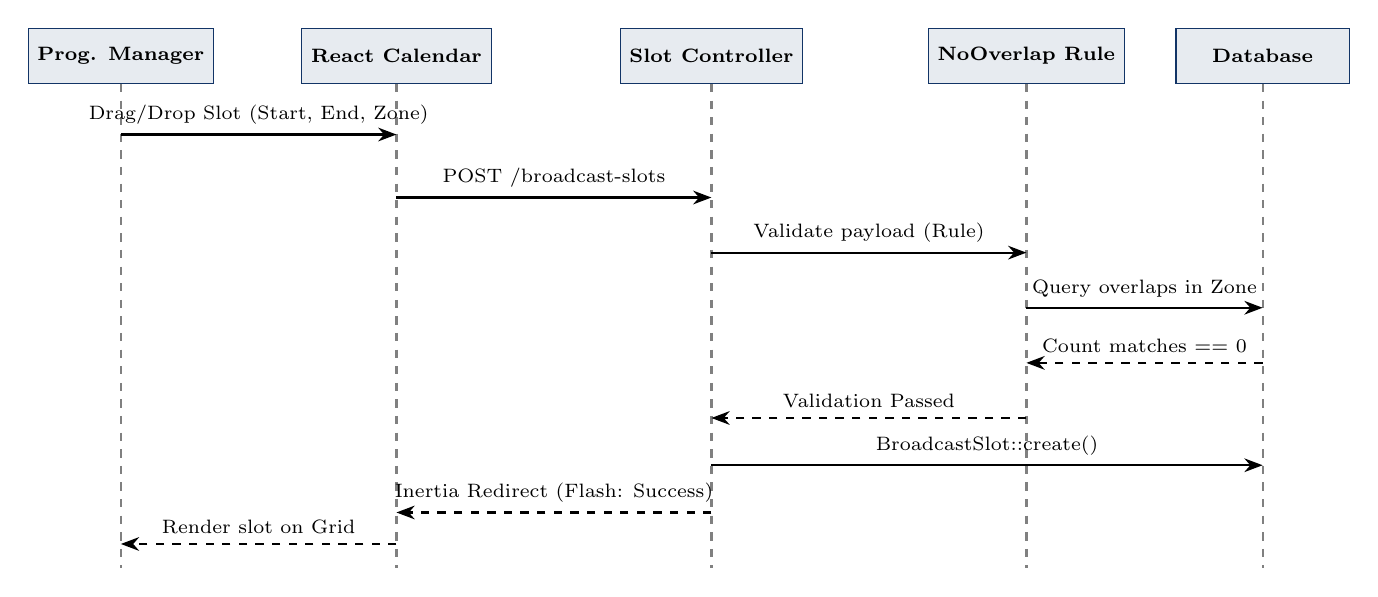
\begin{tikzpicture}[
    lifeline/.style={draw=gray, dashed, thick},
    msg/.style={-Stealth, thick, font=\scriptsize},
    returnmsg/.style={-Stealth, dashed, thick, font=\scriptsize},
    box/.style={draw=primaryblue, fill=primaryblue!10, minimum width=2.2cm, minimum height=0.7cm, align=center, font=\scriptsize\bfseries}
]
    % Entities
    \node (user) [box] at (0, 0) {Prog. Manager};
    \node (ui) [box] at (3.5, 0) {React Calendar};
    \node (ctrl) [box] at (7.5, 0) {Slot Controller};
    \node (rule) [box] at (11.5, 0) {NoOverlap Rule};
    \node (db) [box] at (14.5, 0) {Database};

    % Lifelines
    \draw[lifeline] (user) -- (0, -6.5);
    \draw[lifeline] (ui) -- (3.5, -6.5);
    \draw[lifeline] (ctrl) -- (7.5, -6.5);
    \draw[lifeline] (rule) -- (11.5, -6.5);
    \draw[lifeline] (db) -- (14.5, -6.5);

    % Messages
    \draw[msg] (0, -1) -- node[above] {Drag/Drop Slot (Start, End, Zone)} (3.5, -1);
    \draw[msg] (3.5, -1.8) -- node[above] {POST /broadcast-slots} (7.5, -1.8);
    \draw[msg] (7.5, -2.5) -- node[above] {Validate payload (Rule)} (11.5, -2.5);
    \draw[msg] (11.5, -3.2) -- node[above] {Query overlaps in Zone} (14.5, -3.2);
    \draw[returnmsg] (14.5, -3.9) -- node[above] {Count matches == 0} (11.5, -3.9);
    \draw[returnmsg] (11.5, -4.6) -- node[above] {Validation Passed} (7.5, -4.6);
    \draw[msg] (7.5, -5.2) -- node[above] {BroadcastSlot::create()} (14.5, -5.2);
    \draw[returnmsg] (7.5, -5.8) -- node[above] {Inertia Redirect (Flash: Success)} (3.5, -5.8);
    \draw[returnmsg] (3.5, -6.2) -- node[above] {Render slot on Grid} (0, -6.2);
\end{tikzpicture}
\caption{Sequence Diagram: Broadcast Slot Creation with Interval Overlap Verification}
\label{fig:seq_slot}
\end{figure}

\subsection{Sequence Diagram 2: AI Assistant Query Execution with Live RAG Context}
This sequence demonstrates the dynamic retrieval-augmented generation pattern enabling GridCast AI to provide real-time responses.

\begin{figure}[h!]
\centering
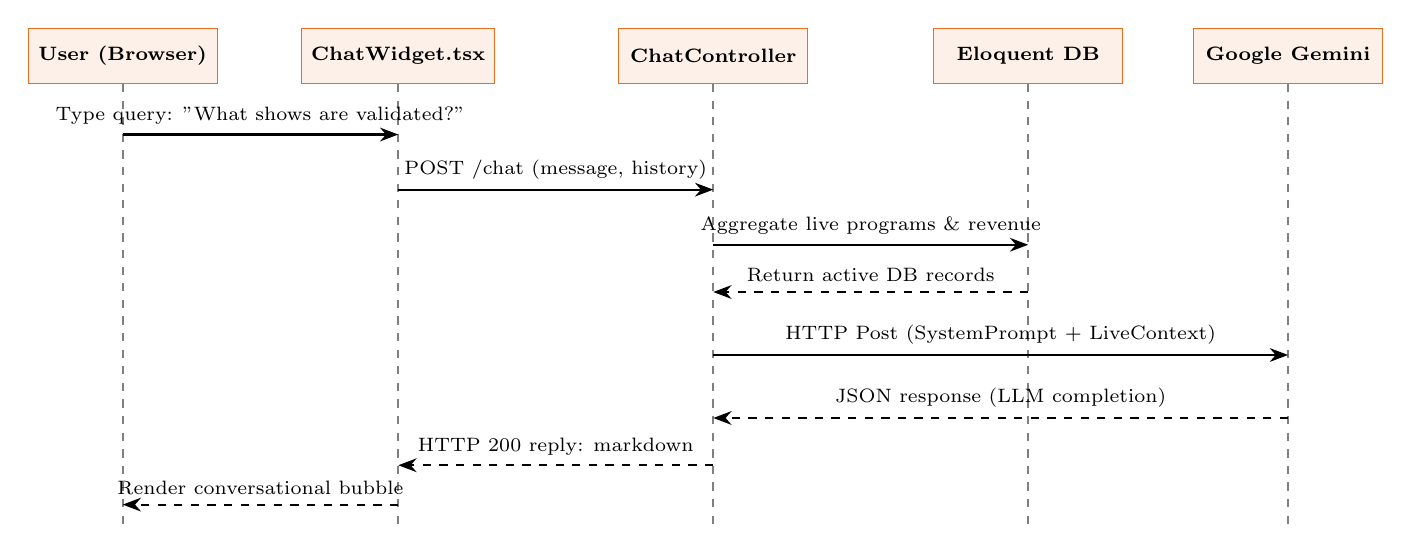
\begin{tikzpicture}[
    lifeline/.style={draw=gray, dashed, thick},
    msg/.style={-Stealth, thick, font=\scriptsize},
    returnmsg/.style={-Stealth, dashed, thick, font=\scriptsize},
    box/.style={draw=accentorange, fill=accentorange!10, minimum width=2.4cm, minimum height=0.7cm, align=center, font=\scriptsize\bfseries}
]
    \node (user) [box] at (0, 0) {User (Browser)};
    \node (widget) [box] at (3.5, 0) {ChatWidget.tsx};
    \node (ctrl) [box] at (7.5, 0) {ChatController};
    \node (db) [box] at (11.5, 0) {Eloquent DB};
    \node (gemini) [box] at (14.8, 0) {Google Gemini};

    \draw[lifeline] (user) -- (0, -6.0);
    \draw[lifeline] (widget) -- (3.5, -6.0);
    \draw[lifeline] (ctrl) -- (7.5, -6.0);
    \draw[lifeline] (db) -- (11.5, -6.0);
    \draw[lifeline] (gemini) -- (14.8, -6.0);

    \draw[msg] (0, -1.0) -- node[above] {Type query: "What shows are validated?"} (3.5, -1.0);
    \draw[msg] (3.5, -1.7) -- node[above] {POST /chat (message, history)} (7.5, -1.7);
    \draw[msg] (7.5, -2.4) -- node[above] {Aggregate live programs \& revenue} (11.5, -2.4);
    \draw[returnmsg] (11.5, -3.0) -- node[above] {Return active DB records} (7.5, -3.0);
    \draw[msg] (7.5, -3.8) -- node[above] {HTTP Post (SystemPrompt + LiveContext)} (14.8, -3.8);
    \draw[returnmsg] (14.8, -4.6) -- node[above] {JSON response (LLM completion)} (7.5, -4.6);
    \draw[returnmsg] (7.5, -5.2) -- node[above] {HTTP 200 {reply: markdown}} (3.5, -5.2);
    \draw[returnmsg] (3.5, -5.7) -- node[above] {Render conversational bubble} (0, -5.7);
\end{tikzpicture}
\caption{Sequence Diagram: AI Assistant Live RAG Contextual Inquiry}
\label{fig:seq_ai}
\end{figure}

\section{Static Structural Modeling: Class Diagram}
Figure~\ref{fig:class_diagram} outlines the domain entities and their relational cardinality in GridCast.

\begin{figure}[h!]
\centering
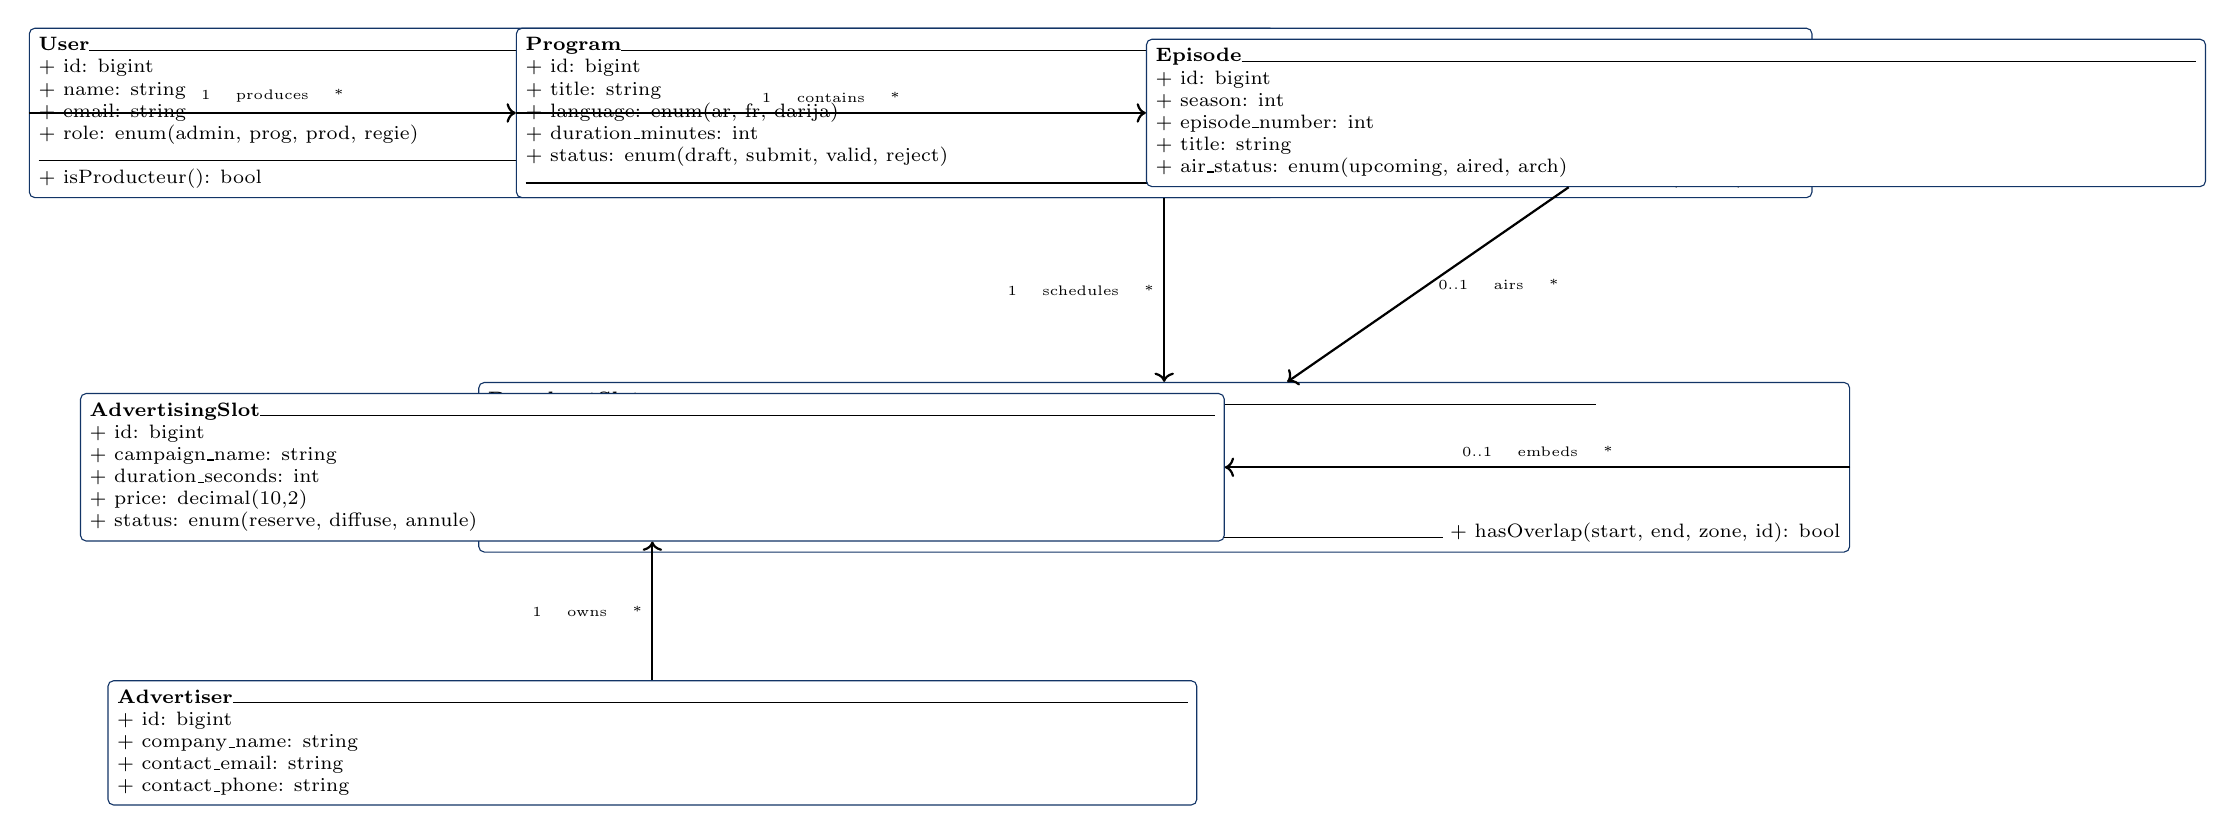
\begin{tikzpicture}[
    classbox/.style={draw=primaryblue, fill=white, rounded corners=2pt, minimum width=4cm, font=\scriptsize, align=left}
]
    % User
    \node (user) [classbox] at (0, 4) {
        \textbf{\centering User}\rule{\linewidth}{0.4pt}\\
        + id: bigint\\
        + name: string\\
        + email: string\\
        + role: enum(admin, prog, prod, regie)\\
        \rule{\linewidth}{0.4pt}
        + isProgrammation(): bool\\
        + isProducteur(): bool
    };

    % Program
    \node (prog) [classbox] at (6.5, 4) {
        \textbf{\centering Program}\rule{\linewidth}{0.4pt}\\
        + id: bigint\\
        + title: string\\
        + language: enum(ar, fr, darija)\\
        + duration\_minutes: int\\
        + status: enum(draft, submit, valid, reject)\\
        \rule{\linewidth}{0.4pt}
        + canTransitionTo(status): bool
    };

    % Episode
    \node (ep) [classbox] at (13, 4) {
        \textbf{\centering Episode}\rule{\linewidth}{0.4pt}\\
        + id: bigint\\
        + season: int\\
        + episode\_number: int\\
        + title: string\\
        + air\_status: enum(upcoming, aired, arch)
    };

    % BroadcastSlot
    \node (slot) [classbox] at (6.5, -0.5) {
        \textbf{\centering BroadcastSlot}\rule{\linewidth}{0.4pt}\\
        + id: bigint\\
        + start\_datetime: datetime\\
        + end\_datetime: datetime\\
        + channel\_zone: string\\
        + slot\_type: enum(emission, pub)\\
        \rule{\linewidth}{0.4pt}
        + hasOverlap(start, end, zone, id): bool
    };

    % AdvertisingSlot
    \node (adslot) [classbox] at (0, -0.5) {
        \textbf{\centering AdvertisingSlot}\rule{\linewidth}{0.4pt}\\
        + id: bigint\\
        + campaign\_name: string\\
        + duration\_seconds: int\\
        + price: decimal(10,2)\\
        + status: enum(reserve, diffuse, annule)
    };

    % Advertiser
    \node (adv) [classbox] at (0, -4) {
        \textbf{\centering Advertiser}\rule{\linewidth}{0.4pt}\\
        + id: bigint\\
        + company\_name: string\\
        + contact\_email: string\\
        + contact\_phone: string
    };

    % Relationships
    \draw[->, thick] (user) -- node[above, font=\tiny] {1 \quad produces \quad *} (prog);
    \draw[->, thick] (prog) -- node[above, font=\tiny] {1 \quad contains \quad *} (ep);
    \draw[->, thick] (prog) -- node[left, font=\tiny] {1 \quad schedules \quad *} (slot);
    \draw[->, thick] (ep) -- node[right, font=\tiny] {0..1 \quad airs \quad *} (slot);
    \draw[->, thick] (slot) -- node[above, font=\tiny] {0..1 \quad embeds \quad *} (adslot);
    \draw[->, thick] (adv) -- node[left, font=\tiny] {1 \quad owns \quad *} (adslot);
\end{tikzpicture}
\caption{UML Domain Class Diagram}
\label{fig:class_diagram}
\end{figure}


% ==============================================================================
% CHAPTER 4: IMPLEMENTATION AND TECHNICAL REALIZATION
% ==============================================================================
\chapter{Implementation and Technical Realization}
\label{chap:impl}

\section{Introduction}
This chapter provides an exhaustive technical breakdown of the implementation phase of GridCast, detailing the architectural choices, concrete code structures, quality guarantees, and user experience components developed during the internship.

\section{System Architecture: Modern Monolithic SPA with Inertia.js}
Modern full-stack web engineering frequently struggles with the trade-offs of microservices or decoupled client-server applications. While separate Single-Page Applications (e.g., pure React consuming a REST or GraphQL API) provide dynamic user interfaces, they introduce significant friction: duplicate schema declarations, complex client-side state managers, authentication token synchronizations (JWT), and elevated latency.

GridCast resolves this dilemma by deploying \textbf{Inertia.js v2}. Inertia acts as a seamless protocol bridging Laravel 12 on the server with React 19 on the client:
\begin{itemize}
    \item Routing and business rules reside entirely on the backend in PHP.
    \item Laravel controllers return \texttt{Inertia::render('PageName', \$props)}, delivering Eloquent model data directly into the React tree.
    \item Inertia intercepts internal hyperlinks, replacing standard browser page reloads with lightweight XHR requests that exchange JSON state, yielding instantaneous client-side navigation.
\end{itemize}

\begin{figure}[h!]
\centering
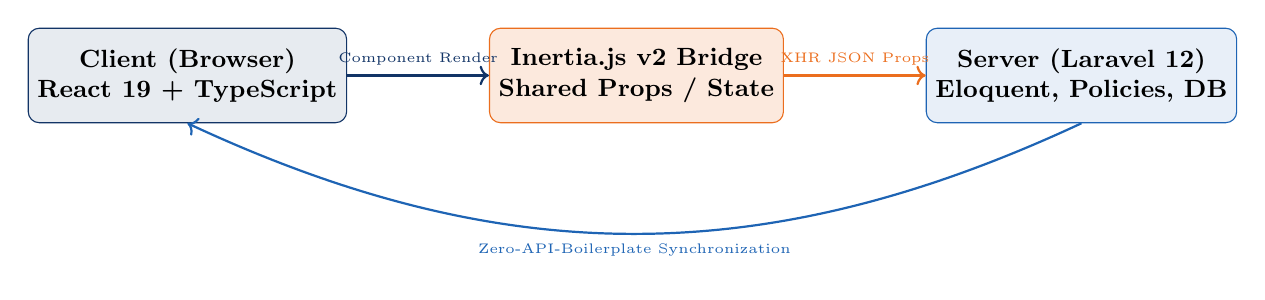
\begin{tikzpicture}[node distance=1cm, auto]
    \node (browser) [draw=primaryblue, fill=primaryblue!10, rounded corners, minimum width=3.5cm, minimum height=1.2cm, align=center, font=\small\bfseries] {Client (Browser)\\React 19 + TypeScript};
    \node (inertia) [draw=accentorange, fill=accentorange!15, rounded corners, minimum width=3.5cm, minimum height=1.2cm, right=1.8cm of browser, align=center, font=\small\bfseries] {Inertia.js v2 Bridge\\Shared Props / State};
    \node (laravel) [draw=secondaryblue, fill=secondaryblue!10, rounded corners, minimum width=3.5cm, minimum height=1.2cm, right=1.8cm of inertia, align=center, font=\small\bfseries] {Server (Laravel 12)\\Eloquent, Policies, DB};

    \draw[->, thick, color=primaryblue] (browser.east) -- (inertia.west) node[midway, above, font=\tiny] {Component Render};
    \draw[->, thick, color=accentorange] (inertia.east) -- (laravel.west) node[midway, above, font=\tiny] {XHR JSON Props};
    \draw[<-, thick, color=secondaryblue] (browser.south) to[bend right=25] node[midway, below, font=\tiny] {Zero-API-Boilerplate Synchronization} (laravel.south);
\end{tikzpicture}
\caption{Inertia.js Monolithic SPA Architectural Topology}
\label{fig:inertia_arch}
\end{figure}

\section{Core Backend Implementation (Laravel 12)}

\subsection{Temporal Overlap Prevention Logic}
The non-overlap constraint is implemented via a dedicated validation rule (\texttt{NoBroadcastOverlap.php}) and encapsulated within the \texttt{BroadcastSlot} model. Two time intervals $[S_1, E_1]$ and $[S_2, E_2]$ overlap if and only if:
\begin{equation}
    (S_1 < E_2) \quad \land \quad (E_1 > S_2)
\end{equation}

Listing~\ref{lst:overlap_php} demonstrates the query implemented in the Eloquent model:
\begin{lstlisting}[language=PHP, caption={Broadcast Slot Overlap Detection Query in Laravel 12}, label={lst:overlap_php}]
public static function hasOverlap(
    string $start, 
    string $end, 
    string $channelZone, 
    ?int $excludeId = null
): bool {
    return self::where('channel_zone', $channelZone)
        ->where('start_datetime', '<', $end)
        ->where('end_datetime', '>', $start)
        ->when($excludeId, fn ($q) => $q->where('id', '!=', $excludeId))
        ->exists();
}
\end{lstlisting}

\subsection{Program Lifecycle State Machine}
To enforce governance over audiovisual submissions, transitions are validated on the backend:
\begin{lstlisting}[language=PHP, caption={Program State Machine Transition Logic}, label={lst:state_machine}]
public function canTransitionTo(string $newStatus): bool
{
    return match ($this->status) {
        self::STATUS_BROUILLON => in_array($newStatus, [self::STATUS_SOUMIS]),
        self::STATUS_SOUMIS    => in_array($newStatus, [self::STATUS_VALIDE, self::STATUS_REJETE]),
        self::STATUS_REJETE    => in_array($newStatus, [self::STATUS_BROUILLON]),
        self::STATUS_VALIDE    => false, // Validated programs cannot be altered
        default                => false,
    };
}
\end{lstlisting}

\section{Frontend Engineering (React 19, TypeScript \& Tailwind v4)}

\subsection{Interactive Weekly Schedule Grid with @dnd-kit}
The weekly planning calendar was constructed using the modular drag-and-drop library \texttt{@dnd-kit/core}. The grid renders seven vertical columns representing the days of the week, divided into half-hour broadcast increments. Placed broadcast slots utilize draggable hooks (\texttt{useDraggable}), while target hourly slots implement droppable targets (\texttt{useDroppable}). Upon dropping a slot, an asynchronous request is dispatched to the backend, which executes the overlap check before updating the calendar state.

\subsection{Data Analytics Visualization with Recharts}
The executive dashboard embeds responsive SVG data visualizations via \texttt{recharts}:
\begin{itemize}
    \item \textbf{Category Distribution (PieChart):} Visualizes audiovisual balance (News, Series, Sports, Documentaries, Religion).
    \item \textbf{Audience by Transmission Zone (BarChart):} Displays average viewers across Prime Time, Access, and Matinée.
\end{itemize}

\section{Real-Time AI Assistant Integration (Gemini 2.5 Flash)}
To provide conversational access to GridCast data, the system integrates \textbf{Google Gemini 2.5 Flash} via a server-side controller (\texttt{ChatController.php}).

Rather than querying a static language model with no knowledge of Moroccan television schedules, GridCast utilizes a **dynamic RAG injection pattern**:
\begin{enumerate}
    \item Upon receiving a query, the backend computes an operational snapshot: total programs, approval counts, upcoming broadcasts for the next 72 hours, registered advertisers, and total advertising revenue.
    \item This live context is injected into the Gemini \texttt{systemInstruction} payload alongside behavioral rules.
    \item The client renders the streaming markdown response within an accessible floating React drawer (\texttt{ChatWidget.tsx}).
\end{enumerate}

\section{Quality Assurance and Testing}
Automated tests were written using the \textbf{Pest PHP} framework:
\begin{itemize}
    \item \texttt{ProgramPolicyTest.php}: Verifies role-based access restrictions.
    \item \texttt{BroadcastSlotOverlapTest.php}: Asserts that overlapping time slots in the same zone are rejected, while adjacent or cross-zone slots are accepted.
    \item \texttt{ProgramWorkflowTest.php}: Asserts state machine integrity.
    \item \texttt{ControllerCrudTest.php}: Verifies end-to-end CRUD operations.
\end{itemize}

Code hygiene was enforced using \texttt{composer run lint} (Laravel Pint adhering to PSR-12) and \texttt{npm run lint} (ESLint flat config with TypeScript).


% ==============================================================================
% CHAPTER 5: DEVOPS PIPELINE AND DEPLOYMENT ARCHITECTURE
% ==============================================================================
\chapter{DevOps Pipeline and Deployment Architecture}
\label{chap:devops}

\section{Introduction}
Television broadcast infrastructures cannot tolerate unplanned outages. Delivering high availability and reproducibility requires a modern DevOps deployment strategy. This chapter details the containerization, continuous integration, and infrastructure architecture designed for GridCast.

\section{Containerization Architecture with Docker}
GridCast is packaged using multi-container Docker topologies orchestrated via Docker Compose.

\subsection{Multi-Stage Production Dockerfile}
To minimize production image size and eliminate development dependencies, a multi-stage Docker build was engineered (Listing~\ref{lst:dockerfile}).

\begin{lstlisting}[language=bash, caption={Production Multi-Stage Dockerfile for GridCast}, label={lst:dockerfile}]
# Stage 1: Build Frontend Assets
FROM node:22-alpine AS frontend-builder
WORKDIR /app
COPY package*.json ./
RUN npm ci
COPY . .
RUN npm run build

# Stage 2: PHP Application Container
FROM php:8.2-fpm-alpine AS backend
WORKDIR /var/www/html

# Install System & PHP Extensions
RUN apk add --no-cache nginx supervisor mysql-client libpng-dev libzip-dev \
    && docker-php-ext-install pdo_mysql bcmath gd zip opcache

# Install Composer
COPY --from=composer:2.7 /usr/bin/composer /usr/bin/composer

# Copy Source Code & Frontend Build Artifacts
COPY . .
COPY --from=frontend-builder /app/public/build ./public/build

# Install Production Dependencies & Optimize
RUN composer install --no-dev --optimize-autoloader --no-interaction
RUN php artisan config:cache && php artisan route:cache && php artisan view:cache

EXPOSE 80 9000
CMD ["supervisord", "-c", "/etc/supervisor/conf.d/supervisord.conf"]
\end{lstlisting}

\subsection{Multi-Container Orchestration (Docker Compose)}
The system orchestrates four dedicated service containers:
\begin{enumerate}
    \item \textbf{App/Web Container:} Nginx + PHP 8.2-FPM running the Laravel application.
    \item \textbf{Database Container:} MySQL 8.0 with persistent storage volumes.
    \item \textbf{Cache \& Queue Service:} Redis 7.2 for session persistence and asynchronous job queuing.
    \item \textbf{Queue Worker Daemon:} Dedicated worker managed by Supervisor executing broadcast notifications and analytics batch jobs.
\end{enumerate}

\section{Continuous Integration and Continuous Deployment (CI/CD)}
A production-grade CI/CD pipeline was constructed using GitHub Actions (Listing~\ref{lst:cicd}).

\begin{figure}[h!]
\centering
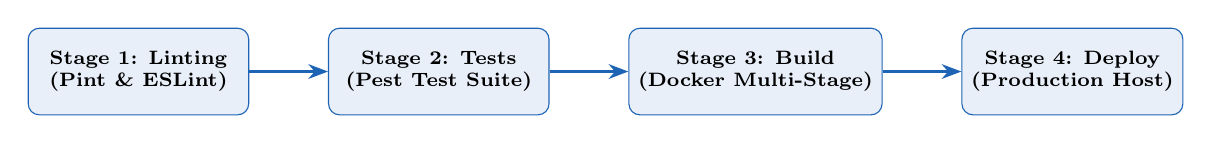
\begin{tikzpicture}[
    stage/.style={draw=secondaryblue, fill=secondaryblue!10, rounded corners, minimum width=2.8cm, minimum height=1.1cm, align=center, font=\scriptsize\bfseries},
    arrow/.style={-{Stealth[length=2.5mm]}, thick, color=secondaryblue}
]
    \node (lint) [stage] {Stage 1: Linting\\(Pint \& ESLint)};
    \node (test) [stage, right=1cm of lint] {Stage 2: Tests\\(Pest Test Suite)};
    \node (build) [stage, right=1cm of test] {Stage 3: Build\\(Docker Multi-Stage)};
    \node (deploy) [stage, right=1cm of build] {Stage 4: Deploy\\(Production Host)};

    \draw[arrow] (lint) -- (test);
    \draw[arrow] (test) -- (build);
    \draw[arrow] (build) -- (deploy);
\end{tikzpicture}
\caption{Continuous Integration and Deployment Pipeline Flow}
\label{fig:cicd_flow}
\end{figure}

\begin{lstlisting}[language=yaml, caption={GitHub Actions CI/CD Pipeline Configuration (.github/workflows/deploy.yml)}, label={lst:cicd}]
name: GridCast CI/CD Pipeline

on:
  push:
    branches: [ main ]
  pull_request:
    branches: [ main ]

jobs:
  code-quality:
    runs-on: ubuntu-latest
    steps:
      - uses: actions/checkout@v4
      - name: Setup PHP
        uses: shivammathur/setup-php@v2
        with:
          php-version: '8.2'
      - name: Check PSR-12 Linting
        run: vendor/bin/pint --test
      - name: Check Frontend Linting
        run: npm ci && npm run lint

  automated-testing:
    needs: code-quality
    runs-on: ubuntu-latest
    steps:
      - uses: actions/checkout@v4
      - name: Execute Pest Tests
        run: php artisan test --stop-on-failure

  docker-build-and-deploy:
    needs: automated-testing
    if: github.ref == 'refs/heads/main'
    runs-on: ubuntu-latest
    steps:
      - name: Build and Push Docker Image
        uses: docker/build-push-action@v5
        with:
          push: true
          tags: registry.liongeek.ma/gridcast:latest
      - name: Deploy via SSH
        uses: appleboy/ssh-action@master
        with:
          host: \${{ secrets.PROD_SERVER_IP }}
          username: deploy
          key: \${{ secrets.SSH_PRIVATE_KEY }}
          script: |
            cd /opt/gridcast && docker compose pull && docker compose up -d
            docker compose exec -T app php artisan migrate --force
\end{lstlisting}

\section{Production Infrastructure and Security Hardening}
\begin{itemize}
    \item \textbf{Reverse Proxy \& TLS Encryption:} Incoming web requests terminate at an Nginx reverse proxy secured by Let's Encrypt SSL/TLS certificates with strict HTTP Strict Transport Security (HSTS) headers.
    \item \textbf{Process Supervision:} Supervisor monitors background queue workers, restarting failed worker processes automatically.
    \item \textbf{Automated Backup Automation:} Nightly automated database dumps are stored in S3-compatible object storage with 30-day retention policies.
\end{itemize}

\newpage

% ==============================================================================
% CONCLUSION AND FUTURE PERSPECTIVES
% ==============================================================================
\chapter*{Conclusion and Future Perspectives}
\addcontentsline{toc}{chapter}{Conclusion and Future Perspectives}

\section*{Retrospective Assessment}
The two-month internship conducted at \textbf{LionGeek}, the digital innovation subsidiary of \textbf{SOREAD 2M}, was an enriching and formative engineering milestone. Immersed within the operational environment of Morocco's leading national broadcaster, I was granted the opportunity to tackle real-world television engineering challenges.

The initial two weeks of on-site technical immersion provided the foundation necessary to master the full-stack ecosystem of \textbf{Laravel 12}, \textbf{Inertia.js v2}, \textbf{React 19}, and \textbf{Tailwind CSS v4}. Concurrently contributing to a high-priority confidential enterprise project under non-disclosure constraints provided firsthand exposure to corporate software engineering standards and enterprise-level data confidentiality.

The primary project, \textbf{GridCast}, successfully achieved all initial requirements:
\begin{itemize}
    \item Designed an interactive weekly television grid with mathematical interval overlap protection.
    \item Implemented a trilingual audiovisual program catalog supporting Arabic, Darija, and French metadata.
    \item Established an audiovisual submission lifecycle with strict state machine validation.
    \item Created a commercial advertising module tracking revenue metrics.
    \item Integrated an intelligent conversational assistant (\textbf{GridCast AI}) powered by Google Gemini 2.5 Flash using live database RAG context injection.
    \item Established a complete DevOps deployment blueprint incorporating multi-stage Docker builds and automated CI/CD pipelines.
\end{itemize}

\section*{Future Perspectives}
While GridCast delivers a functional operational foundation, several perspectives emerge for future development:
\begin{enumerate}
    \item \textbf{Live HLS Video Ingestion \& Preview:} Integrating an embedded video player allowing programming executives to preview broadcast files directly on the scheduling interface.
    \item \textbf{Predictive Audience Forecasting:} Employing machine learning models trained on historical viewership data to predict prime-time ratings prior to final schedule validation.
    \item \textbf{Automated SCTE-35 Commercial Cue Markers:} Automatically inserting digital ad cue-tone markers into the broadcast playout automation feed to synchronize digital streaming advertising with terrestrial television breaks.
\end{enumerate}

\newpage

% ==============================================================================
% REFERENCES & WEBOGRAPHY
% ==============================================================================
\begin{thebibliography}{99}
\addcontentsline{toc}{chapter}{References \& Webography}

\bibitem{laravel_docs}
Taylor Otwell et al.
\newblock \emph{Laravel 12 Documentation: The PHP Framework for Web Artisans}.
\newblock \url{https://laravel.com/docs/12.x}, 2025.

\bibitem{inertia_docs}
Jonathan Reinink.
\newblock \emph{Inertia.js v2 Documentation: The Modern Monolith}.
\newblock \url{https://inertiajs.com/}, 2025.

\bibitem{react_docs}
Meta Open Source.
\newblock \emph{React 19 Reference Documentation}.
\newblock \url{https://react.dev/}, 2025.

\bibitem{gemini_api}
Google DeepMind.
\newblock \emph{Gemini 2.5 Flash: Generative AI Developer Documentation}.
\newblock \url{https://ai.google.dev/docs}, 2025.

\bibitem{pest_php}
Nuno Maduro.
\newblock \emph{Pest PHP: Elegant Testing Framework for PHP}.
\newblock \url{https://pestphp.com/}, 2025.

\bibitem{tailwind_docs}
Adam Wathan et al.
\newblock \emph{Tailwind CSS v4: Rapid UI Styling}.
\newblock \url{https://tailwindcss.com/}, 2025.

\bibitem{docker_docs}
Docker Inc.
\newblock \emph{Docker Containerization Best Practices and Multi-Stage Builds}.
\newblock \url{https://docs.docker.com/}, 2025.

\bibitem{fowler_enterprise}
Martin Fowler.
\newblock \emph{Patterns of Enterprise Application Architecture}.
\newblock Addison-Wesley Professional, 2002.

\bibitem{ehtp_guidelines}
Hassania School of Public Works (EHTP).
\newblock \emph{Engineering Internship Guidelines and Academic Thesis Framework}.
\newblock Casablanca, Morocco, 2025.

\end{thebibliography}

\end{document}
